\documentclass[10pt,letterpaper]{article}
% ---------------------------------------------------------------------------
% Laboratorio 7 - CC3092 Deep Learning y Sistemas Inteligentes
% Compilar desde la raiz del repositorio:
%   latexmk -pdf -cd informe/informe.tex
% ---------------------------------------------------------------------------
\usepackage[spanish,es-noshorthands,es-tabla]{babel}
\usepackage[T1]{fontenc}
\usepackage{lmodern}
\usepackage{microtype}
\usepackage[letterpaper,margin=1.6cm,top=1.4cm,bottom=1.45cm]{geometry}
\usepackage{amsmath,amssymb}
\usepackage{graphicx}
\usepackage{booktabs}
\usepackage{tabularx}
\usepackage{multirow}
\usepackage{float}
\usepackage[font=footnotesize,labelfont=bf,skip=3pt]{caption}
\usepackage{subcaption}
\usepackage{enumitem}
\usepackage[table]{xcolor}
\usepackage{fancyhdr}
\usepackage{titlesec}
\usepackage{siunitx}
\usepackage[hidelinks]{hyperref}

\graphicspath{{../figures/}}

\definecolor{acento}{HTML}{1F5F99}
\definecolor{gris}{HTML}{5F6B73}
\definecolor{fondo}{HTML}{F3F5F7}
\hypersetup{colorlinks=true, linkcolor=acento, urlcolor=acento, citecolor=acento}

\titleformat{\section}{\normalsize\bfseries\color{acento}}{\thesection.}{0.5em}{}
\titleformat{\subsection}{\small\bfseries}{\thesubsection}{0.5em}{}
\titlespacing*{\section}{0pt}{0.7em}{0.25em}
\titlespacing*{\subsection}{0pt}{0.5em}{0.15em}

\setlist{itemsep=1pt, topsep=2pt, parsep=0pt, leftmargin=12pt}
\setlength{\parskip}{3pt}
\setlength{\parindent}{0pt}
\setlength{\tabcolsep}{3.5pt}
\setlength{\textfloatsep}{6pt}
\setlength{\floatsep}{5pt}
\setlength{\intextsep}{5pt}
\sisetup{group-separator={,}, group-minimum-digits=4}

\newcommand{\code}[1]{\texttt{#1}}
\newcommand{\repo}{\url{https://github.com/anthonylouschwank/Lab7-DL}}

\pagestyle{fancy}
\fancyhf{}
\renewcommand{\headrulewidth}{0.3pt}
\fancyhead[L]{\footnotesize\color{gris}CC3092 · Laboratorio 7: NLP end-to-end y Embeddings}
\fancyhead[R]{\footnotesize\color{gris}Anthony Lou Schwank}
\fancyfoot[C]{\footnotesize\thepage}
\setlength{\emergencystretch}{2em}


\begin{document}

\begin{center}
  {\small\color{gris}CC3092 Deep Learning y Sistemas Inteligentes}\\[2pt]
  {\Large\bfseries Laboratorio 7: NLP end-to-end y Embeddings}\\[3pt]
  Anthony Lou Schwank \quad·\quad Carné 23410 \quad·\quad Octubre 2026
\end{center}

\vspace{-4pt}
\noindent\colorbox{fondo}{\parbox{\dimexpr\textwidth-2\fboxsep}{\small
\textbf{Resumen.} Se construyó el pipeline texto$\to$tokens$\to$IDs$\to$embeddings$\to$clasificador sobre 30\,M tokens de
WikiText-103. Un skip-gram con negative sampling (SGNS) implementado desde cero en PyTorch alcanza 48.9\,\% en las
analogías de Mikolov y $\rho=0.674$ en WordSim-353, prácticamente igual que Word2Vec de gensim con la misma
configuración (49.0\,\%, 0.669), y 16.6 puntos por debajo de GloVe (6\,B tokens), brecha que se explica en buena parte por
el tamaño del corpus. En AG News, los embeddings preentrenados con \emph{fine-tuning} superan a los aleatorios
(F1 0.914--0.918 vs.\ 0.906) y con 1\,\% de los datos los superan por 15--16 puntos, aunque con todos los datos el baseline
TF-IDF (0.921) sigue siendo el mejor.}}

\section{Investigación: embeddings en PyTorch y gensim}
\begin{itemize}
  \item \code{nn.Embedding(num\_embeddings, embedding\_dim, padding\_idx, sparse)}: tabla entrenable $V\times d$; recibe IDs y
  devuelve sus filas. \code{padding\_idx} fija una fila en cero sin gradiente (para \code{<pad>}); \code{sparse=True}
  produce gradientes sólo de las filas usadas (clave con $V\approx10^5$; requiere \code{SGD}/\code{SparseAdam}/\code{Adagrad}).
  \code{nn.Embedding.from\_pretrained(M, freeze)} crea la tabla desde una matriz (GloVe, SGNS); \code{freeze=True} la congela
  (\code{requires\_grad=False}) y \code{freeze=False} permite \emph{fine-tuning}.
  \item \code{nn.EmbeddingBag(..., mode)} agrega bolsas de vectores sin materializar el tensor $(B,L,d)$: recibe todos los IDs
  concatenados y \code{offsets} (inicio de cada documento), así que no necesita padding. \code{mean} promedia (invariante a la
  longitud), \code{sum} suma (admite \code{per\_sample\_weights}) y \code{max} toma el máximo por dimensión.
  \item \textbf{gensim}: \code{Word2Vec} (\code{vector\_size}, \code{window}, \code{min\_count}, \code{sg}, \code{negative},
  \code{sample}, \code{alpha}, \code{epochs}); \code{KeyedVectors} ofrece \code{most\_similar} (3CosAdd), \code{most\_similar\_cosmul},
  \code{evaluate\_word\_analogies}, \code{evaluate\_word\_pairs} y \code{save\_word2vec\_format}.
  \item \textbf{CBOW vs.\ skip-gram}: CBOW predice la palabra central desde el promedio del contexto (rápido, favorece palabras
  frecuentes); skip-gram predice cada contexto desde la central (más pares por token, mejor con palabras raras y analogías).
  \item \textbf{Dos matrices}: $W$ (palabra como centro) y $W'$ (palabra como contexto/negativo). Con una sola matriz el modelo
  debería dar baja probabilidad a $\sigma(v_w^\top v_w)$, que es siempre grande, y la optimización se degrada. Se conserva $W$.
  \item \textbf{Word2Vec vs.\ GloVe}: Word2Vec es \emph{predictivo} (SGD local sobre ventanas, contexto real vs.\ negativos);
  GloVe es \emph{de conteo}: construye la matriz global $X_{ij}$ y ajusta $w_i^\top\tilde w_j+b_i+\tilde b_j\approx\log X_{ij}$
  por mínimos cuadrados ponderados. SGNS factoriza implícitamente una PMI desplazada (Levy \& Goldberg, 2014).
\end{itemize}

\section{Exploración y preprocesamiento}
\textbf{Corpus.} El split \code{train} de WikiText-103 tiene \num{1801350} líneas (\num{1165029} no vacías, de las cuales
\num{275630} son encabezados de sección), \num{29444} líneas de título de artículo (el dataset reporta \num{28475}
artículos; el resto son líneas con el mismo formato \code{" = X = "}) y \num{101425671} tokens separados por espacios
(\num{84593278} tras nuestra normalización, que elimina la puntuación; \num{717430} tipos).

\textbf{Normalización (alineada con GloVe 6B, \emph{uncased} y tokenizado estilo PTB).}
(i)~minúsculas; (ii)~se reconstruyen los artefactos de WikiText (\code{well @-@ known}$\to$\code{well-known},
\code{1 @,@ 000}$\to$\code{1,000}, \code{1 @.@ 5}$\to$\code{1.5}); (iii)~contracciones PTB (\code{didn 't}$\to$\code{did n't},
\code{can't}$\to$\code{ca n't}, \code{'s} separado); (iv)~compuestos con guion y siglas/abreviaturas con punto
(\code{u.s.}, \code{dr.}, \code{jan.}) como un solo token; (v)~números como dígitos (sin \code{<num>}); (vi)~puntuación
eliminada (no aparece en los benchmarks y ocuparía posiciones de la ventana). En los embeddings las palabras bajo
\code{min\_count} se \emph{eliminan} antes de formar ventanas (como Word2Vec); en clasificación no se necesita \code{<pad>}
porque \code{EmbeddingBag} usa \code{offsets}. Lo que \emph{debe} coincidir con GloVe es el casing, el formato de contracciones,
guiones y números: si no, una misma palabra tendría formas distintas y los benchmarks se evaluarían sobre preguntas diferentes.

\textbf{Tokenizador propio vs.\ librerías} (12 oraciones, sin puntuación). Coincide con NLTK salvo en siglas finales
(\code{u.s.} vs.\ \code{u.s}, \code{e.g.}), \code{i'd've} (NLTK deja \code{i'd}) y correos. spaCy difiere más: parte los
compuestos con guion (\code{state | of | the | art}, \code{york | based}, \code{10 | 15}), quita el punto de \code{dr.}/\code{jan.}
y conserva \code{jsmith@example.com}. Las tres separan igual \code{ca n't}, \code{wo n't} e \code{is n't}.


\begin{figure}[H]
\centering
\begin{minipage}[c]{0.43\textwidth}
  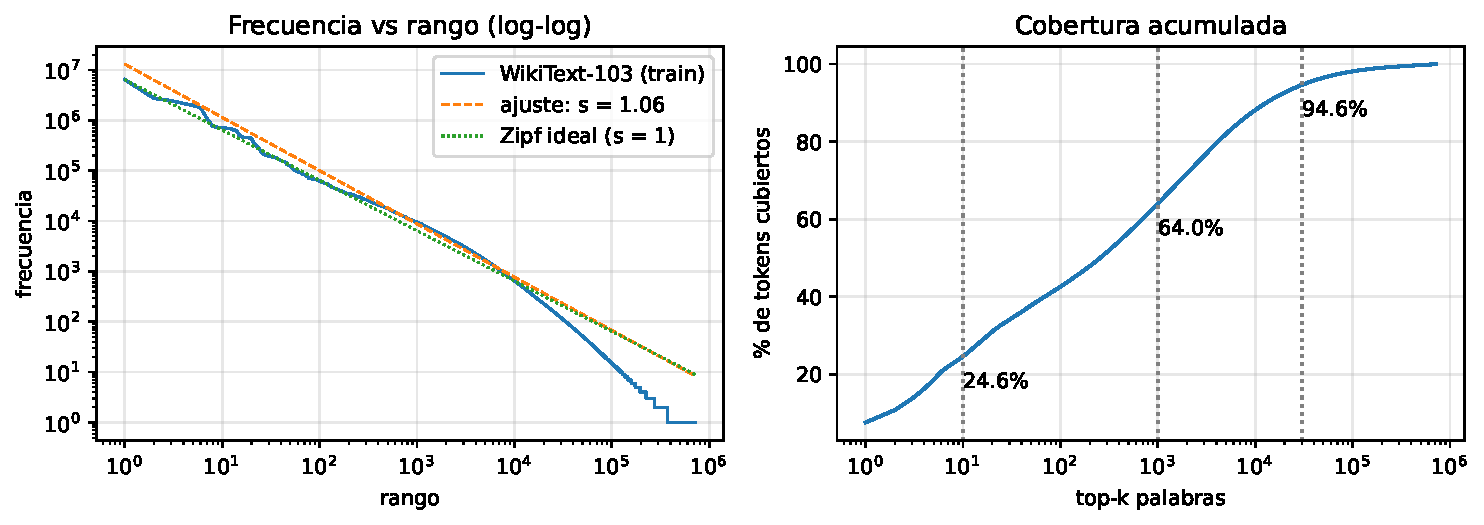
\includegraphics[width=\linewidth]{zipf.pdf}
\end{minipage}\hfill
\begin{minipage}[c]{0.555\textwidth}
\footnotesize
\begin{tabular}{@{}rrr@{\hspace{8pt}}lrrr@{}}
\toprule
\code{min\_count} & $|V|$ & \% desc. & palabra & $t{=}10^{-3}$ & $t{=}10^{-4}$ & $t{=}10^{-5}$ \\
\midrule
1  & \num{392765} & 0.00 & \code{the} & 87.3 & 96.3 & 98.8 \\
3  & \num{153008} & 0.98 & \code{of}  & 79.5 & 94.2 & 98.2 \\
5  & \num{109700} & 1.47 & \code{and} & 78.2 & 93.8 & 98.1 \\
10 & \num{72652}  & 2.28 & corpus    & 22.6 & 39.9 & 64.1 \\
20 & \num{48370}  & 3.38 & \multicolumn{4}{l}{\scriptsize (\% de apariciones descartadas)}\\
50 & \num{27810}  & 5.51 & & & & \\
\bottomrule
\end{tabular}
\end{minipage}
\caption{Izq.: ley de Zipf en WikiText-103 (85\,M tokens). Der.: vocabulario y \% de tokens desconocidos por
\code{min\_count} en el subconjunto de 30\,M tokens, y \% de apariciones descartadas por el submuestreo.}
\label{fig:zipf}
\end{figure}

\textbf{Zipf, vocabulario y submuestreo.} La curva rango-frecuencia es casi una recta en log-log con exponente
$s=1.06$ (ajuste en rangos 10--\num{10000}): se cumple la ley de Zipf, con desviación en la cola (hápax). Las 10, \num{1000}
y \num{30000} palabras más frecuentes cubren 24.6\,\%, 64.0\,\% y 94.6\,\% de los tokens. Elegimos \code{min\_count}$=5$:
$|V|=\num{109700}$ con sólo 1.5\,\% de tokens perdidos (la mayoría, nombres raros y errores). Con la fórmula de Word2Vec
$P_\text{keep}=(\sqrt{f/t}+1)\,t/f$ y $t=10^{-4}$ se descarta el 96\,\% de \code{the} y el 94\,\% de \code{of}/\code{and}
(40\,\% del corpus). Ayuda porque esas palabras aportan poca información sobre sus vecinas, reduce los pares a la mitad y,
al quitarlas antes de formar ventanas, éstas abarcan más palabras de contenido. \textbf{Pares skip-gram} (ventana 5, sin
cruzar párrafos): 286.6\,M por epoch con ventana fija y 173.1\,M con ventana dinámica ($b\sim U\{1..5\}$) antes del
submuestreo; 168.8\,M y \textbf{102.4\,M} después (17.8\,M tokens conservados).

\section{Construcción y entrenamiento de los embeddings}
\textbf{SGNS propio.} Dos tablas \code{nn.Embedding(sparse=True)} ($W\sim U(\pm0.5/d)$, $W'=0$), pérdida
$-\log\sigma(u_o^\top v_c)-\sum_{k}\log\sigma(-u_{n_k}^\top v_c)$ con negativos de $P_n\propto\text{count}^{0.75}$, \code{SparseAdam}
con batch \num{8192} y decaimiento lineal del lr. Como Word2Vec: submuestreo nuevo en cada epoch, ventana dinámica y
ventanas sin cruzar párrafos; los pares se generan en GPU por bloques de 2\,M tokens y se barajan. \textbf{gensim}: mismo
archivo de corpus, mismo \code{min\_count} (vocabulario idéntico) y mismos \code{window}, \code{negative}, \code{sample},
\code{vector\_size}, \code{epochs}; el lr no es equivalente (SGD $0.025\to10^{-4}$), así que se dejó el de gensim.
\textbf{Selección} sólo con WordSim-353 y analogías (top-\num{30000} de cada modelo, como \code{restrict\_vocab}):
score $=(\text{acc}_\text{analogías}+\rho_\text{WS})/2$. El evaluador propio en GPU reproduce exactamente a gensim
(GloVe: 0.6549 y 0.5327). Primero se barrió el lr y luego se varió un factor a la vez; la combinación ganadora sólo
cambió los negativos ($K=15$) y se reentrenó con 10 epochs.

\begin{table}[H]
\centering\footnotesize
\begin{tabular}{@{}lrrrrrrrrrrrrrr@{}}
\toprule
Iteración & tokens & $|V|$ & $d$ & win & $K$ & $t$ & lr & ep & pérdida & sem & sin & total & WS-353 & s/epoch \\
\midrule
lr $2{\times}10^{-3}$ & 30.0\,M & 109.7k & 100 & 5 & 5 & $10^{-4}$ & 0.002 & 5 & 2.173 & .283 & .452 & .401 & .665 & 43 \\
\textbf{base} (lr $5{\times}10^{-3}$) & 30.0\,M & 109.7k & 100 & 5 & 5 & $10^{-4}$ & 0.005 & 5 & 2.140 & .387 & .471 & .446 & .674 & 52 \\
lr $10^{-2}$ & 30.0\,M & 109.7k & 100 & 5 & 5 & $10^{-4}$ & 0.01 & 5 & 2.136 & .404 & .468 & .449 & .666 & 62 \\
$d=50$ & 30.0\,M & 109.7k & 50 & 5 & 5 & $10^{-4}$ & 0.005 & 5 & 2.189 & .251 & .390 & .349 & .635 & 47 \\
$d=300$ & 30.0\,M & 109.7k & 300 & 5 & 5 & $10^{-4}$ & 0.005 & 5 & 2.057 & .523 & .483 & .495 & .663 & 199 \\
ventana 2 & 30.0\,M & 109.7k & 100 & 2 & 5 & $10^{-4}$ & 0.005 & 5 & 2.008 & .328 & .483 & .437 & .656 & 106 \\
ventana 10 & 30.0\,M & 109.7k & 100 & 10 & 5 & $10^{-4}$ & 0.005 & 5 & 2.205 & .418 & .461 & .448 & .668 & 242 \\
$K=2$ & 30.0\,M & 109.7k & 100 & 5 & 2 & $10^{-4}$ & 0.005 & 5 & 1.491 & .342 & .447 & .416 & \textbf{.684} & 181 \\
$K=15$ & 30.0\,M & 109.7k & 100 & 5 & 15 & $10^{-4}$ & 0.005 & 5 & 3.046 & .448 & .486 & .475 & .671 & 293 \\
$t=10^{-3}$ & 30.0\,M & 109.7k & 100 & 5 & 5 & $10^{-3}$ & 0.005 & 5 & 2.184 & .376 & .494 & .458 & .655 & 280 \\
$t=10^{-5}$ & 30.0\,M & 109.7k & 100 & 5 & 5 & $10^{-5}$ & 0.005 & 5 & 2.047 & .394 & .399 & .397 & .668 & 125 \\
\code{min\_count}$=10$ & 30.0\,M & 72.7k & 100 & 5 & 5 & $10^{-4}$ & 0.005 & 5 & 2.170 & .377 & .474 & .445 & .674 & 104 \\
corpus 25\,\% & 7.5\,M & 50.3k & 100 & 5 & 5 & $10^{-4}$ & 0.005 & 5 & 2.133 & .172 & .247 & .224 & .618 & 48 \\
corpus 50\,\% & 15.0\,M & 74.7k & 100 & 5 & 5 & $10^{-4}$ & 0.005 & 5 & 2.134 & .324 & .396 & .374 & .651 & 86 \\
\textbf{mejor} ($K{=}15$, 10 ep) & 30.0\,M & 109.7k & 100 & 5 & 15 & $10^{-4}$ & 0.005 & 10 & 3.028 & \textbf{.474} & \textbf{.496} & \textbf{.490} & .674 & 277 \\
\midrule
gensim (mejor cfg) & 30.0\,M & 109.7k & 100 & 5 & 15 & $10^{-4}$ & SGD & 10 & --- & .461 & .502 & .490 & .669 & 101$^\dagger$ \\
\bottomrule
\end{tabular}
\caption{Iteraciones (métricas al final del entrenamiento; analogías sobre las \num{30000} palabras más frecuentes de
cada modelo). Memoria GPU pico: 2.1--3.5\,GB (3.1\,GB con $d=300$). $^\dagger$CPU, 8 hilos. Los tiempos están inflados
y son ruidosos: la GPU (RTX 3070 Laptop) entró en \emph{throttling} térmico y compartió recursos con otros procesos
(las primeras epochs tardaban $\approx$36\,s). Tiempo total del mejor SGNS: 46\,min; gensim: 17\,min.}
\label{tab:iter}
\end{table}

\begin{figure}[H]
\centering
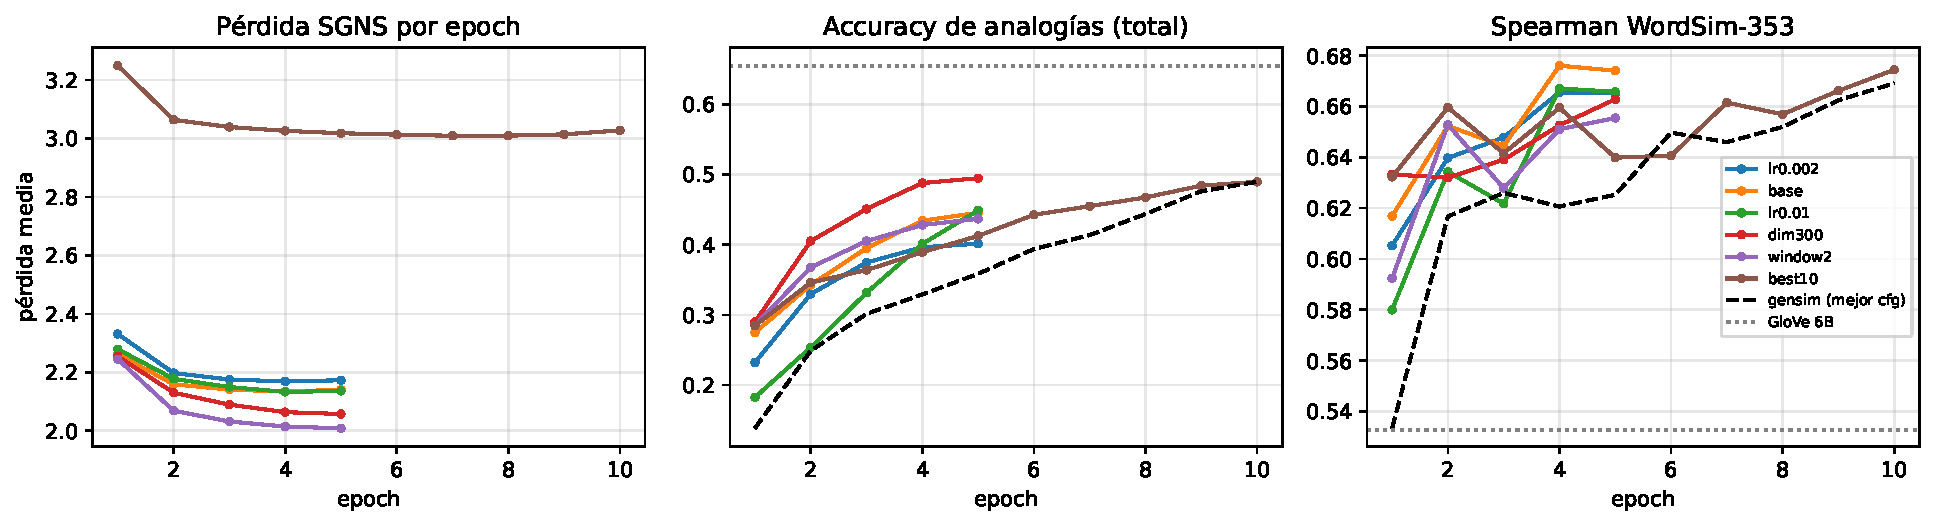
\includegraphics[width=\textwidth]{curvas_entrenamiento.pdf}
\caption{Pérdida, accuracy de analogías y Spearman en WordSim-353 por epoch para 6 iteraciones y gensim (línea negra).}
\label{fig:curvas}
\end{figure}

\textbf{¿Menor pérdida $\Rightarrow$ mejores embeddings? No.} La pérdida depende de la tarea: $K=2$ tiene la menor
pérdida (1.49) y la ventana 2 la segunda (2.01), y ambas dan peores analogías que la base; $K=15$ tiene pérdida 3.05 y es
la mejor. Incluso dentro de una corrida la pérdida del mejor modelo \emph{sube} de 3.010 (epoch 8) a 3.028 (epoch 10)
mientras las analogías mejoran de 46.7 a 48.9\,\%. Los vecinos de control se vuelven coherentes desde la epoch 2
(\code{france}$\to$\code{spain, italy, belgium}; \code{computer}$\to$\code{computers, software, computing};
\code{january}$\to$ otros meses); \code{king} queda dominado por nombres de reyes raros (\code{osric}, \code{wenceslaus}), un
efecto del corpus enciclopédico que gensim también muestra.

\section{Verificación de la aritmética vectorial}
\textbf{Analogías individuales.} \code{analogia(a,b,c,k)} usa 3CosAdd, $\arg\max_x\cos(x,\hat b-\hat a+\hat c)$, sobre
vectores normalizados (top-\num{100000}) excluyendo $a,b,c$. Devuelve las mismas palabras y cosenos que
\code{most\_similar} de gensim en los tres modelos. Se probaron 20 analogías propias de 7 tipos. Aciertos top-1: SGNS 15/20,
gensim 14/20, GloVe 17/20. Todos aciertan gentilicios, tiempos verbales (\code{go:went::take:took}), comparativos y plurales
regulares. Los fallos más ilustrativos (rango de la respuesta): \code{man:king::woman:queen} (SGNS 2, gensim 5, GloVe 1; SGNS
propone \code{jagiellon} con 0.74 vs.\ \code{queen} 0.73); \code{canada:ottawa::australia:canberra} (250 / 120 / 2: Canberra
aparece poco en 30\,M tokens); \code{mouse:mice::foot:feet} (76 / 36 / 1); \code{big:biggest::small:smallest} (11 / 6 / 11; todos
proponen \code{large/largest}) y \code{possible:impossible::legal:illegal} (589 / 165 / 268). El coseno entre el vector
resultado y la respuesta correcta nunca es 1: 0.73 (SGNS), 0.69 (gensim) y 0.77 (GloVe) para \code{queen}.

\textbf{Sin excluir la consulta}, la primera palabra es $b$ o $c$ en 12/20 (SGNS), 13/20 (gensim) y 9/20 (GloVe) analogías.
Para \code{man:king::woman:?} los tres devuelven \code{king} (0.77, 0.78, 0.84) antes que \code{queen}; para
\code{walk:walked::swim:?} SGNS y gensim devuelven \code{swim}. Es decir, $\hat b-\hat a+\hat c$ suele quedar más cerca de
una palabra de la consulta que de la respuesta: la "aritmética" sólo funciona como búsqueda del vecino más cercano
\emph{después} de excluir esas palabras.

\begin{table}[H]
\centering\footnotesize
\begin{tabular}{@{}lr|rr|rr|rr|ccc@{}}
\toprule
& & \multicolumn{2}{c|}{SGNS propio} & \multicolumn{2}{c|}{gensim} & \multicolumn{2}{c|}{GloVe} & \multicolumn{3}{c}{paralelismo (cos medio)} \\
Categoría & cobert. & Add & Mul & Add & Mul & Add & Mul & SGNS & gensim & GloVe \\
\midrule
capital-common-countries & .75 & .708 & .668 & .729 & .668 & .929 & .911 & .34 & .35 & .58 \\
capital-world & .23 & .571 & .523 & .579 & .521 & .883 & .859 & .25 & .26 & .57 \\
currency & .06 & .019 & .019 & .019 & .019 & .056 & .056 & .28 & .24 & .25 \\
city-in-state & .71 & .361 & .326 & .324 & .299 & .302 & .268 & .18 & .19 & .34 \\
family & .68 & .564 & .503 & .576 & .529 & .880 & .868 & .25 & .25 & .51 \\
adjective-to-adverb & .82 & .121 & .105 & .132 & .113 & .280 & .278 & .12 & .12 & .27 \\
opposite & .34 & .070 & .063 & .143 & .103 & .272 & .239 & .09 & .10 & .23 \\
comparative & 1.00 & .517 & .503 & .578 & .552 & .800 & .781 & .30 & .31 & .42 \\
superlative & .63 & .325 & .313 & .298 & .295 & .608 & .611 & .28 & .28 & .47 \\
present-participle & .82 & .438 & .386 & .430 & .386 & .722 & .716 & .16 & .18 & .32 \\
nationality-adjective & .81 & .865 & .851 & .851 & .826 & .974 & .958 & .47 & .48 & .75 \\
past-tense & .85 & .630 & .597 & .619 & .559 & .588 & .562 & .20 & .20 & .29 \\
plural & .74 & .510 & .457 & .460 & .408 & .799 & .764 & .16 & .16 & .31 \\
plural-verbs & .75 & .335 & .348 & .383 & .385 & .583 & .611 & .26 & .26 & .36 \\
\midrule
\textbf{Semánticas} & .40 & .474 & .433 & .461 & .421 & .590 & .564 & & & \\
\textbf{Sintácticas} & .77 & .496 & .473 & .500 & .469 & .683 & .670 & & & \\
\textbf{Total} & .61 & \textbf{.490} & .461 & .489 & .454 & \textbf{.655} & .638 & .24 {\scriptsize(.12)} & .24 {\scriptsize(.12)} & .40 {\scriptsize(.17)} \\
\bottomrule
\end{tabular}
\caption{Accuracy en \code{questions-words.txt} sobre el vocabulario compartido (las \num{30000} palabras más frecuentes de
nuestro corpus presentes en los tres modelos; \num{11834} de \num{19544} preguntas, 60.6\,\%). Paralelismo: coseno medio entre
todos los pares de vectores diferencia $\hat b-\hat a$ de la categoría; entre paréntesis, la línea base con pares mal
emparejados.}
\label{tab:cat}
\end{table}

\textbf{Evaluación sistemática y paralelismo.} Con las mismas \num{11834} preguntas, SGNS y gensim empatan (48.9\,\%) y
GloVe llega a 65.5\,\%. 3CosMul no mejoró a 3CosAdd en ningún modelo (-2 a -4 puntos) con este vocabulario restringido. Si la
aritmética fuera exacta, los vectores diferencia de una relación serían paralelos (coseno 1); en SGNS el coseno medio es
sólo 0.24 (0.40 en GloVe), aunque el doble de la línea base aleatoria. Las relaciones más paralelas (gentilicios 0.47,
países-capitales 0.34) son justo las de mayor accuracy, y las menos paralelas (opuestos 0.09, adjetivo-adverbio 0.12) las
peores. \textbf{t-SNE} de 479 palabras en 14 grupos temáticos (figura en el notebook): se forman los grupos esperados.
La pureza de los 5 vecinos más cercanos en el espacio original es 0.84 en SGNS y 0.89 en GloVe: meses/días e instrumentos
son perfectos (1.00), números y deportes casi (0.97), y los más mezclados son capitales (0.62, se confunden con países y
ciudades de EE.\,UU.) y profesiones (0.74).

\section{Pipeline end-to-end: clasificación de AG News}
Mismo \code{tokenize} de la sección 2; 10\,\% estratificado de train como validación (\num{108000}/\num{12000}) y test oficial
(\num{7600}) usado una sola vez. Clasificador: \code{EmbeddingBag(mean)} $\to$ Linear(100,256) $\to$ ReLU $\to$ Dropout(0.3)
$\to$ Linear(256,4); Adam ($2{\times}10^{-3}$), batch 256, hasta 8 epochs con \emph{early stopping} por F1 de validación.
Vocabulario aleatorio: palabras de train con frecuencia $\ge2$; preentrenado: palabras del modelo presentes en AG News (las
fuera de vocabulario se descartan). Tokens de AG News (test) fuera de vocabulario: \textbf{SGNS y gensim 3.3\,\%, GloVe
0.8\,\%}. Baseline: TF-IDF de uni+bigramas (\code{min\_df}=2, \code{sublinear\_tf}) + regresión logística ($C=4$ elegido en
validación).

\begin{table}[H]
\centering\footnotesize
\begin{tabular}{@{}lccccrrr|cc@{}}
\toprule
& \multicolumn{4}{c}{Validación (macro)} & & & & \multicolumn{2}{c}{Test (mejor variante)} \\
Modelo & Acc & Prec & Rec & F1 & params totales & entrenables & tiempo & Acc & F1 \\
\midrule
TF-IDF + LogReg & .9248 & .9246 & .9248 & \textbf{.9246} & \num{1698048} & \num{1698048} & 151\,s & \textbf{.9213} & \textbf{.9211} \\
Aleatorio (entrenado) & .9143 & .9145 & .9143 & .9142 & \num{4950084} & \num{4950084} & 6\,s & .9055 & .9055 \\
SGNS congelado & .8856 & .8856 & .8856 & .8854 & \num{4566384} & \num{26884} & 4\,s & & \\
SGNS fine-tuning & .9188 & .9187 & .9188 & .9186 & \num{4566384} & \num{4566384} & 4\,s & .9141 & .9139 \\
gensim congelado & .8868 & .8893 & .8868 & .8867 & \num{4566384} & \num{26884} & 4\,s & & \\
gensim fine-tuning & .9185 & .9195 & .9185 & .9185 & \num{4566384} & \num{4566384} & 5\,s & .9136 & .9136 \\
GloVe congelado & .9036 & .9041 & .9036 & .9036 & \num{6628384} & \num{26884} & 4\,s & & \\
GloVe fine-tuning & .9229 & .9236 & .9229 & .9229 & \num{6628384} & \num{6628384} & 6\,s & .9183 & .9183 \\
\bottomrule
\end{tabular}
\caption{Clasificación de AG News (las curvas de pérdida de entrenamiento y validación están en el notebook).}
\label{tab:clf}
\end{table}

\begin{figure}[H]
\centering
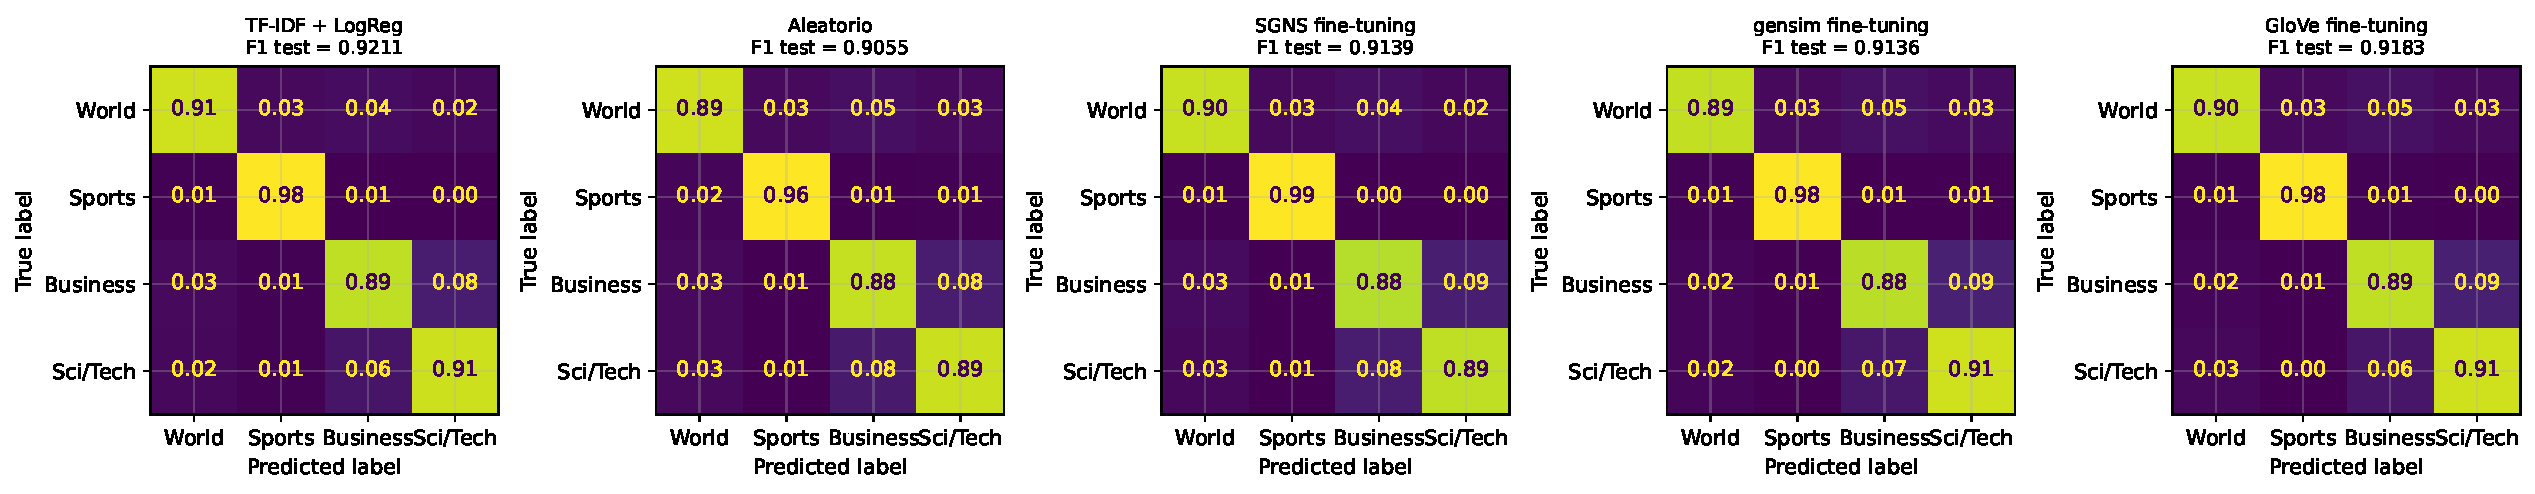
\includegraphics[width=0.8\textwidth]{confusion_test.pdf}
\caption{Matrices de confusión normalizadas en test de la mejor variante de cada inicialización. En todos los modelos la
mayor confusión es Business$\leftrightarrow$Sci/Tech (6--9\,\%) y la clase más fácil es Sports (96--99\,\%).}
\label{fig:conf}
\end{figure}

\textbf{SimLex-999} (reservado hasta el final): $\rho=0.295$ (SGNS), 0.312 (gensim) y 0.298 (GloVe), con cobertura de
99.6--100\,\%. A diferencia de WordSim-353 (que mide \emph{relación}, donde nuestros modelos superan a GloVe: 0.674 vs.\
0.533), SimLex mide \emph{similitud} estricta y penaliza que antónimos y palabras relacionadas compartan contexto: los tres
modelos quedan igual de mal.

\section{Comparación de resultados}
\begin{table}[H]
\centering\footnotesize
\begin{tabular}{@{}lccc@{}}
\toprule
& SGNS propio (PyTorch) & Word2Vec (gensim) & GloVe 6B (preentrenado) \\
\midrule
Tokens / vocabulario / dimensión & 30.0\,M / \num{109700} / 100 & 30.0\,M / \num{109700} / 100 & 6\,B / \num{400000} / 100 \\
Tiempo y hardware & 46\,min, RTX 3070 Laptop (8\,GB) & 17\,min, CPU 8 hilos & $\approx$85\,min co-ocurrencias + 50 iter. \\
& & & (2$\times$ Xeon E5-2658, 32 núcleos) \\
Analogías 3CosAdd (sem / sin / total) & .474 / .496 / \textbf{.490} & .461 / .500 / .489 & .590 / .683 / \textbf{.655} \\
Analogías 3CosMul (sem / sin / total) & .433 / .473 / .461 & .421 / .469 / .454 & .564 / .670 / .638 \\
Spearman WordSim-353 / SimLex-999 & \textbf{.674} / .295 & .669 / \textbf{.312} & .533 / .298 \\
Cos. medio vectores diferencia (base) & .238 (.116) & .241 (.118) & \textbf{.404} (.175) \\
OOV en AG News (test) / F1 test & 3.3\,\% / .9139 & 3.3\,\% / .9136 & \textbf{0.8\,\%} / \textbf{.9183} \\
\bottomrule
\end{tabular}
\caption{Comparación de los tres conjuntos de embeddings. Tiempos de GloVe según Pennington et al.\ (2014).}
\label{tab:comp}
\end{table}

\begin{figure}[H]
\centering
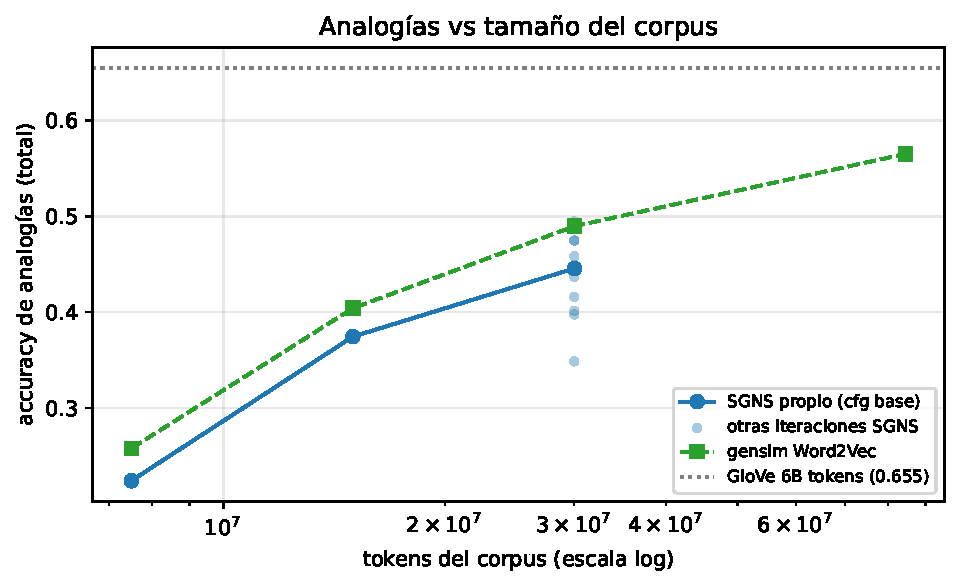
\includegraphics[width=0.49\textwidth]{acc_vs_tokens.pdf}\hfill
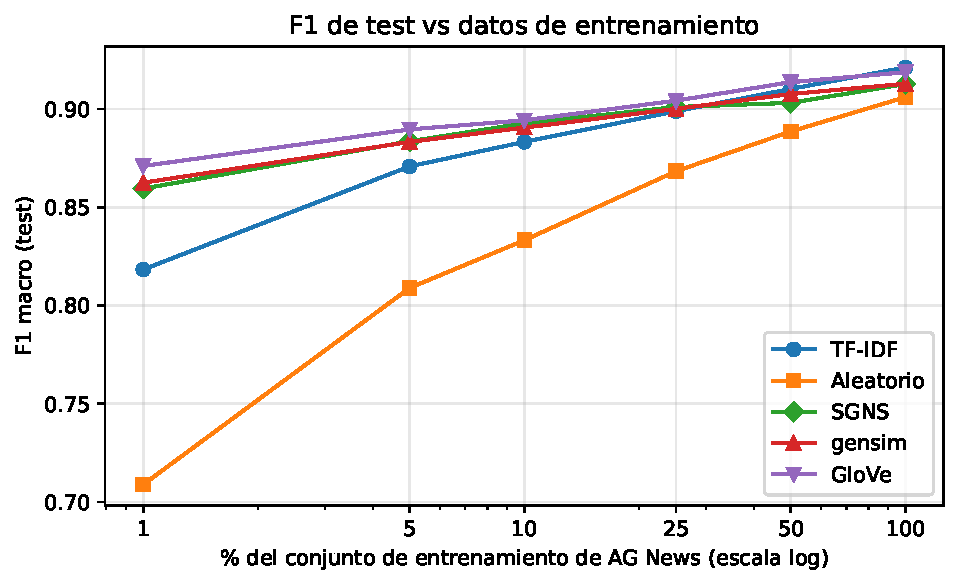
\includegraphics[width=0.49\textwidth]{f1_vs_fraccion.pdf}
\caption{Izq.: accuracy de analogías vs.\ tokens del corpus (escala log) para nuestras iteraciones y gensim (incluye el
split completo de WikiText-103, 85\,M tokens), con GloVe como referencia. Der.: F1 de test vs.\ fracción de AG News usada para
entrenar; para cada inicialización se usa la variante (congelada/fine-tuning) elegida en validación; 1\,\% y 5\,\% promedian 3
semillas.}
\label{fig:escala}
\end{figure}

\section{Discusión y conclusiones}
\textbf{Aritmética vectorial.} Se cumple \emph{aproximadamente}: el mejor SGNS resuelve el 49\,\% de las analogías y 15 de
nuestras 20. Funciona mejor en relaciones morfológicas regulares o muy frecuentes: gentilicios (86\,\%), países-capitales
comunes (71\,\%) y pasado (63\,\%). Falla en monedas (2\,\%, y sólo 6\,\% de cobertura), opuestos (7\,\%) y
adjetivo-adverbio (12\,\%). Las semánticas (47\,\%) quedan un poco por debajo de las sintácticas (50\,\%): las relaciones
semánticas dependen de hechos (qué capital va con qué país) que necesitan ver muchas veces cada par, mientras que la
morfología se aprende con pocos ejemplos frecuentes.

\textbf{¿Es «$\approx$» una igualdad?} No. Sin excluir la consulta, $b$ o $c$ ganan en la mayoría de los casos
(\code{king} queda antes que \code{queen} en los tres modelos), el coseno con la respuesta correcta es 0.7--0.8 y los
vectores diferencia de una misma relación tienen coseno medio 0.24 (0.40 en GloVe), lejos del 1 que implicaría una
igualdad: es un desplazamiento promedio ruidoso, no una identidad.

\textbf{Distancia a GloVe.} 16.6 puntos en analogías. El experimento de corpus indica que la mayor parte se debe a los
datos. Con el mismo método y los mismos hiperparámetros, gensim pasa de 25.8\,\% (7.5\,M) a 40.4\,\% (15\,M), 49.0\,\% (30\,M)
y 56.5\,\% (85\,M). Sólo pasar de 30\,M a 85\,M cierra 7.5 de los 16.6 puntos (45\,\%), y GloVe tiene 70 veces más tokens que
eso, aunque las ganancias por duplicación decrecen (+15, +9 y +5 puntos por duplicación aprox.). El resto se atribuye al
método y a los hiperparámetros: $d=300$ suma 5 puntos, GloVe usa ventana 10, 50 iteraciones y estadísticas globales, y su
vocabulario de 400\,k cubre las palabras raras de las analogías (capital-world: 23\,\% de cobertura en el vocabulario
compartido).

\textbf{SGNS propio vs.\ gensim.} Se comportan casi igual: 48.95\,\% vs.\ 48.96\,\% total, $\rho_\text{WS}$ 0.674 vs.\ 0.669,
paralelismo 0.238 vs.\ 0.241 y F1 en AG News 0.9139 vs.\ 0.9136, con diferencias por categoría de $\pm5$ puntos y los mismos
vecinos atípicos (\code{jagiellon} para \emph{queen}). Las diferencias vienen del optimizador: \code{SparseAdam} con batches de
\num{8192} pares frente al SGD asíncrono por par de gensim. Por eso el nuestro mejora más rápido en las primeras epochs
(Fig.~\ref{fig:curvas}), mientras gensim alcanza el mismo punto al final cuando su lr decae a cero. También influyen el
barajado por bloques y la semilla. La pérdida de gensim no es comparable (se acumula en float32).

\textbf{Hiperparámetros.} \emph{Dimensión}: 50$\to$100$\to$300 da 34.9$\to$44.5$\to$49.5\,\%, sobre todo en semánticas
(25$\to$39$\to$52\,\%), mientras que WordSim se satura en $d=100$. \emph{Ventana}: 2$\to$5$\to$10 sube las semánticas
(32.8$\to$38.7$\to$41.8\,\%) y baja las sintácticas (48.3$\to$47.1$\to$46.1\,\%): \textbf{las ventanas pequeñas favorecen
las relaciones sintácticas} (contexto inmediato: morfología y función) y las grandes, las temáticas o semánticas.
\emph{Negativos}: 2$\to$5$\to$15 da 41.6$\to$44.5$\to$47.5\,\% en analogías, aunque $K=2$ obtuvo el mejor WordSim. Con
$t=10^{-5}$ se descartan demasiadas palabras funcionales y caen las sintácticas (39.9\,\%). Con \code{min\_count}=10 el
resultado es igual con un vocabulario 34\,\% menor. El lr óptimo de \code{SparseAdam} fue $5{\times}10^{-3}$, y duplicar
las epochs sumó 1.5 puntos.

\textbf{AG News.} Los preentrenados con fine-tuning superaron a los aleatorios (F1 test 0.914/0.914/0.918 vs.\ 0.906), pero
\emph{no} al baseline TF-IDF con bigramas (0.921): con \num{108000} ejemplos y clases separables por palabras clave, un modelo
lineal disperso es muy fuerte, y el promedio de embeddings pierde el orden y los bigramas. Con todos los datos conviene el
fine-tuning: congelar cuesta 3--4 puntos, porque la tabla no puede adaptarse a la tarea, aunque entrena 170 veces menos parámetros. \textbf{Con 1\,\% de los datos (\num{1080}
ejemplos) la respuesta cambia}: los preentrenados (SGNS 0.860, GloVe 0.871) superan por 15--16 puntos a los aleatorios
(0.709) y por 4--5 a TF-IDF (0.818), y congelar rinde casi lo mismo que el fine-tuning (GloVe 0.868 vs.\ 0.871, SGNS 0.854
vs.\ 0.860) con mucho menos riesgo de sobreajuste. Los preentrenados sirven sobre todo para aprovechar datos no etiquetados
cuando hay pocas etiquetas. GloVe gana sobre SGNS principalmente por su menor OOV (0.8\,\% vs.\ 3.3\,\%) y
por haber visto noticias (Gigaword).

\textbf{Repositorio:} \repo

\end{document}
